% numerics.tex      pdflatex ZhCvGo15
% Diffuse globally, compute locally: a cyclist tale
% Tingnan Zhang, Daniel I. Goldman and Predrag Cvitanovi\'c

%\subsection{Numerical results}
%                         was {Diffusion in the fundamental domain}
%\label{s-numerics}
\begin{table}[htbp]
	\centering
	\begin{tabular}{|r|r|r|l|l|}
		\hline
		${n_p}$ & \# cycles & $\zeta$(0,0) & $\lambda$ & D \\
		\hline\hline
		1      & 0      &   -    &   -  &   - \\
		2      & 24     & -0.31697 & 1.330 & 0.375\\
		3      & 64     & -0.54152 & 1.435 & 0.339\\
		4      & 168    & -0.09764 & 1.902 & 0.284\\
		5      & 516    &  0.02334 & 2.324 & 0.215\\
		6      & 1589   & -0.00481 & 1.975 & 0.133\\
		7      & 5700   & -0.01241 & 1.885 & 0.184\\
		8      & 20729  & -0.01006 & 1.785 & 0.247\\ \hline
	\end{tabular}
	\caption[Elementary cell cycle expansion results of diffusion coefficient]
        {\label{TCELL1}
        Cycle expansion \refeq{eq-diff-ec} results for the Lyapunov
        exponent $\Lyap$ and the diffusion constant $D$ evaluated in the 		
        elementary cell (as in the 1992 calculation by Schreiber
        \etal\rf{CGS92}).
        }
\end{table}


\begin{table}[htbp]
	\centering
	\begin{tabular}{|r|r|r|l|l|}
		\hline
		$\period{p}$ &
                 \# cycles
                        & $\zeta$(0,0) & $~~~~~\lambda$
                                               & ~~~~~~D \\
		\hline\hline
		1      & 5      & -0.2169759 & 1.39193 & 0.37795 \\
		2      & 10     & -0.0248233 & 1.74541 & 0.23118 \\
		3      & 33     & -0.0221962 & 1.72235 & 0.25257 \\
		4      & 108    & -0.0002192 & 1.74450 & 0.24165 \\
		5      & 373    &  0.0023463 & 1.76079 & 0.24468 \\
		6      & 1378   &  0.0096330 & 1.75610 & 0.24068 \\
		\hline\hline
		\multicolumn{3}{|l|}{numerical experiment}
		& 1.760   & 0.25
		\\ \hline
	\end{tabular}
	\caption[Fundamental domain cycle expansion results of diffusion
	coefficient]{\label{TCELL2}
The Lyapunov exponent $\Lyap$ and the diffusion constant $D$ computed in
the fundamental domain, $w=0.3$ disk-disk separation, disks radius $=1$.
The numerical Lyapunov and diffusion constant are calculated using cycle
averaged mean squared displacement \refeq{eq-fd-msd} on the
elementary cell (see \reffig{fig-disvscont}).
	}
\end{table}

Elementary cell cycles and the corresponding cycle expansion
calculation results are listed in \reftab{TCELL1} (as well as in
~\cite{CGS92}). Using the symbolic
dynamics proposed in~\refsect{s-fundGramm}, we
identify all fundamental periodic orbits up to topolotical length 6,
and list the corresponding calculation results \refeq{eq-fd-msd}
in~\reftab{TCELL2}.
    \PC{2016-07-23} {
    Gaspard 1992 note for \reftab{TCELL2}: ``My numerical estimate for
    the Lyapunov exponent when $w=0.3$ is 		$\lambda = 1.760 \pm
    0.002$, which supports the result of this table.''
        }
    \PC{2016-07-23} { {\bf to Tingnan:}
    Please confirm that the numerical diffusion constant in
    \reftab{TCELL2} is calculated using cycle averaged mean squared
    displacement (MSD) \refeq{eq-fd-msd} on the elementary cell, as in
    \reffig{fig-disvscont}, and not using the Green-Kubo method.
        }
Compared with other methods, the symmetry-reduced cycle expansion method
has the fastest convergence, see \reftab{TCELL2} and
\reffig{fig-convergence}. Diffusion coefficient computed from
$\sim2\,000$ fundamental domain cycles of topological length up to 6
converges with two significant digits, while the elementary cell
calculation needs over $\sim 10\,000$ cycles to show asymptotic behavior.

\begin{figure}
	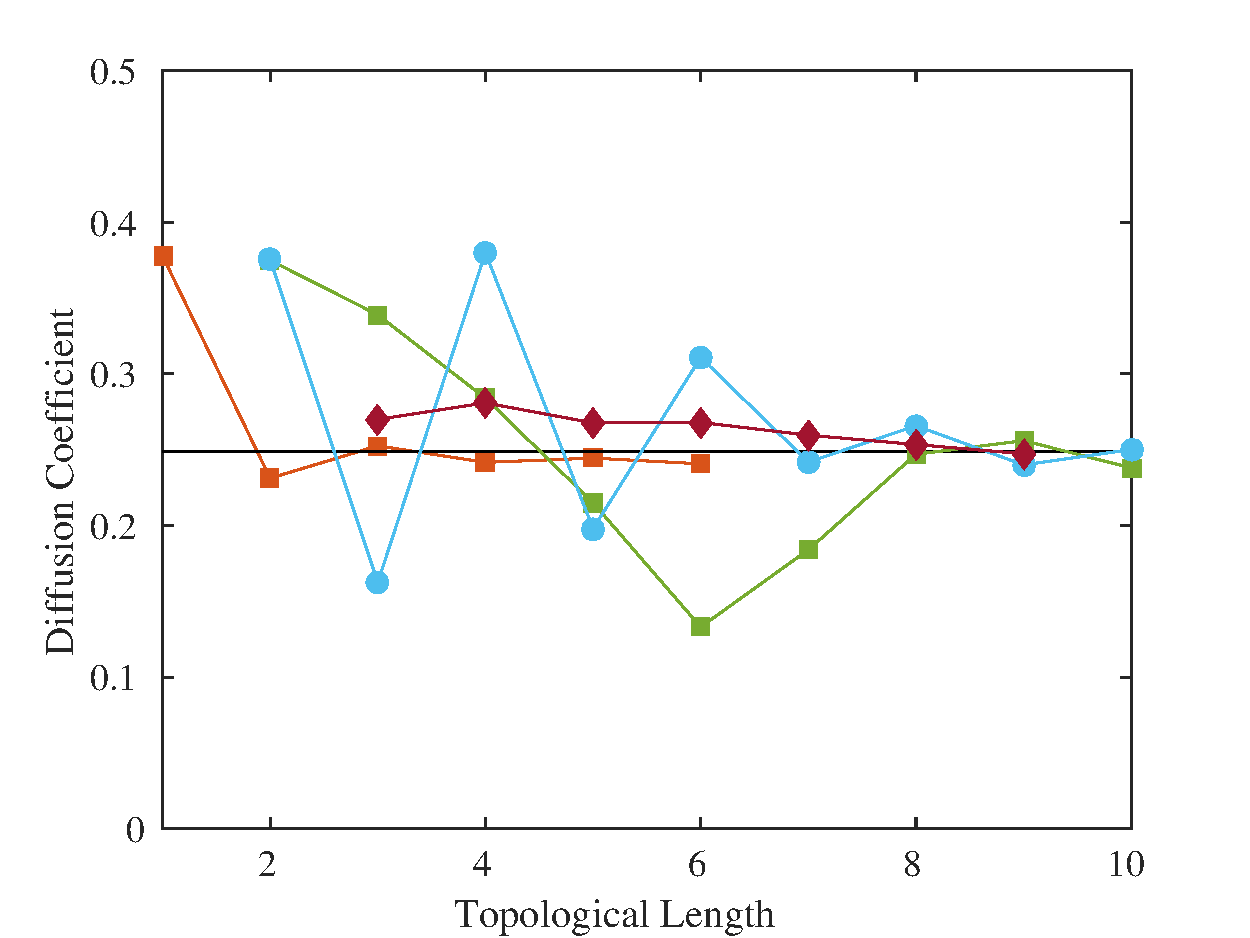
\includegraphics[width=0.5\textwidth]{diffuseCycleExpansionResults}
	\caption{\label{fig-convergence}
The convergence of diffusion constant $D$ \refeq{eq-diff-ec} for  $w=0.3$
disk-disk separation, calculated using cycle expansion in the elementary cell
(green squares) and the fundamental domain (orange squares). Also displayed are
the results of the ``periodic orbit expansion'' method of \refref{MR94}, with and
without Shanks transformation\rf{BenOrs78} (blue circles, crimson diamonds).
		}
\end{figure}

\begin{figure}
	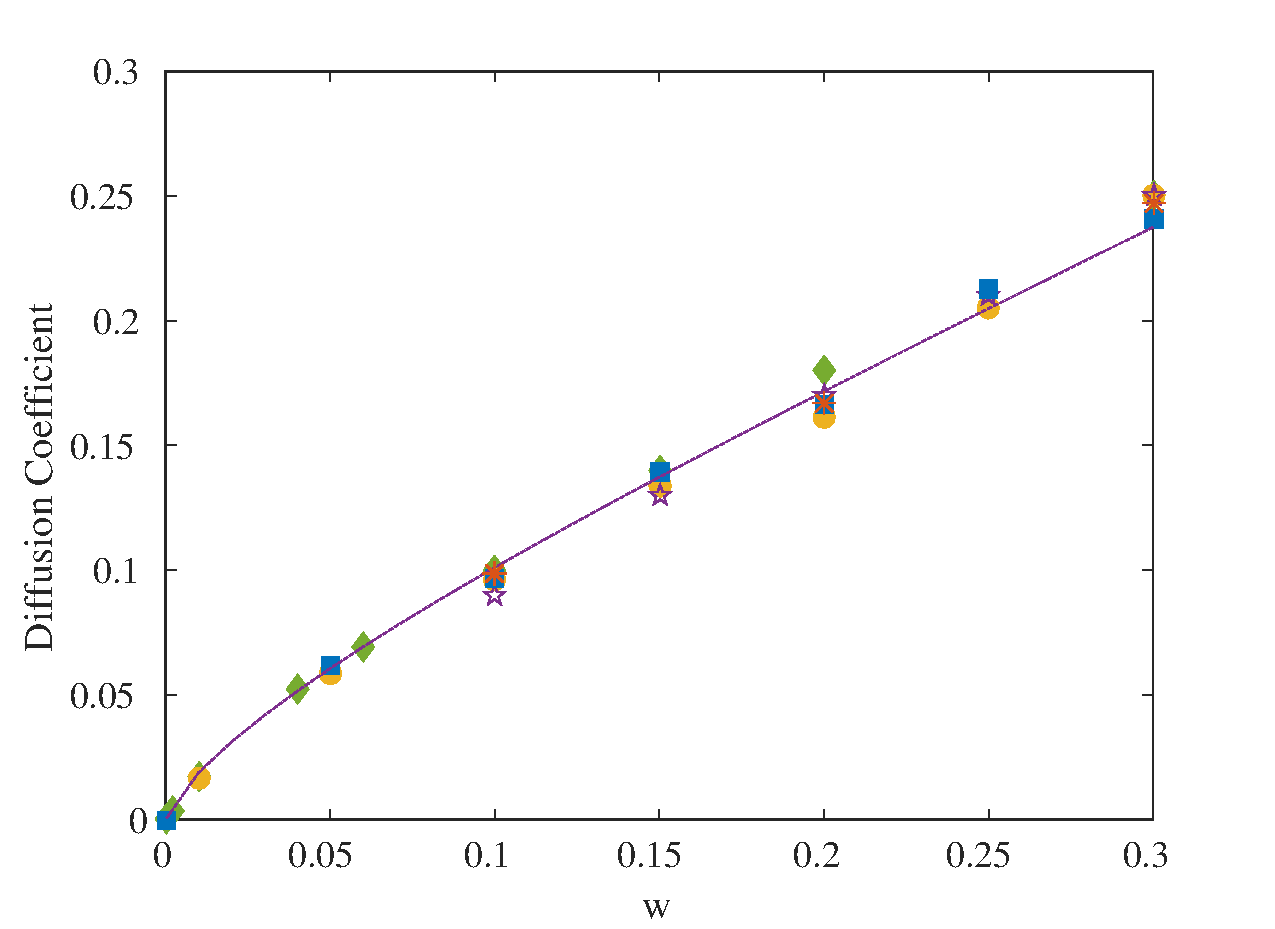
\includegraphics[width=0.5\textwidth]{diffuseDiffCoefPlot}
	\caption[Diffusion coefficients computed using cycle expansion formulas]
    {\label{fig-results}
Diffusion coefficients as a function $w$, compiled from various sources.
Diamonds are Green-Kubo numerical experiments\rf{MacZwa83};
stars\rf{BaEvCo93} and circles\rf{GasBar95} are calculated from the escape
rates; and triangles give the Hausdorff fractal dimension
calculation\rf{GasBar95}. The dashed line  is a statistical approximation
of \refref{AngMor12}.
    }
\end{figure}

We also compute the diffusion constant for different disk-disk separations
$w = 0.05, 0.10, 0.15, 0.20, 0.25, 0.30$.
The results are compared with the earlier numerical estimates and a recent
statistical estimate, in \reffig{fig-results}.
In Green-Kubo velocity auto-correlation method the  diffusion constant can be
extrapolated to the accurate reference value $0.250$ (at $w/r=0.30$), with an
ensemble of $10^6\sim10^7$ random trajectories\rf{MacZwa83}.
The topological length for each trajectory is typically greater than $20$,
significantly larger than what we use in cycle expansion.
On the other hand, while statistical approach yields a smooth analytical
formula\rf{AngMor12}, the diffusion property in such systems is fundamentally
never a smooth function of parameters\rf{KlaDor95}.
Regrettably, our numerical calculations do not have sufficient precision to
display the fractal behavior of diffusion constant, such as what is  observed in
\refref{Cristad06}.

\begin{table}[htbp]
	\centering
	\begin{tabular}{|r|r|r|r||}
		\hline
		$\period{p}$ & \# cycles & D (cont) & D (discrete) \\
		\hline\hline
		1      & 5      & 0.21597 & 0.37795 \\
		2      & 10     & 0.23557 & 0.23118 \\
		3      & 33     & 0.20404 & 0.25257 \\
		4      & 108    & 0.23073 & 0.24165 \\
		5      & 373    & 0.21379 & 0.24468 \\
		6      & 1378   & 0.21902 & 0.24068 \\
		\hline
	\end{tabular}
	\caption[Fundamental domain cycle expansion results of diffusion
	coefficient]{\label{TCELL3}
		Fundamental domain cycle expansion results of diffusion
		coefficient, computed using continuous integral (3rd column)
		and discrete sum (4th column). Here $w = 0.3$.
	}
\end{table}

We have numerically computed the diffusion constant using the map
version of the trace formula. However, if we consider the continuous
flow, i.e. by replacing the discrete sum with the
integral~\refeq{eq-orbitsum}, the result could be different. We find
that the continuous version of the trace formula
converged to lower numerical values ($\sim0.21$ vs. $\sim0.24$,
\reftab{TCELL3}).
To see the
reason, consider the bouncing mode between the nearest disks, cycle
$\{{\bar{0}, \underline{5}}\}$ (\reffig{fig-twodisk}). If the
particle starts at the symmetry line,
the displacement in full space is $0$ after we complete the
fundamental domain cycle once. To the contrary, starting from the
disk edge would generate a net displacement of $w$. A careful
evaluation of the continuous average produce
$\left\langle\vert\hat{L}_{\tp}(1,\tx)\vert^2\right\rangle_{\tp} =
w^2/3$. The situation stands true for every
length-1 fundamental domain periodic orbit---the cycle averaged
square displacement is lower if we count all the points along the
flight. Although the difference between the integral and the discrete
sum vanishes when cycles grow longer, the expansion results are
dominated by the shortest orbits, which contribute exponentially many
times in the formula.

The discrepancy between
the discrete and continuous versions of the cycle expansion is
unclear at this stage. We have also verified the mean square
displacements numerically, using both the map and the flow. The
results are similar, \reffig{fig-disvscont}.

\TZ{2016-06-16}{I think I can try to zoom in the case when $N=1$ and
show if there is a systematic discrepancy.}


\begin{figure}
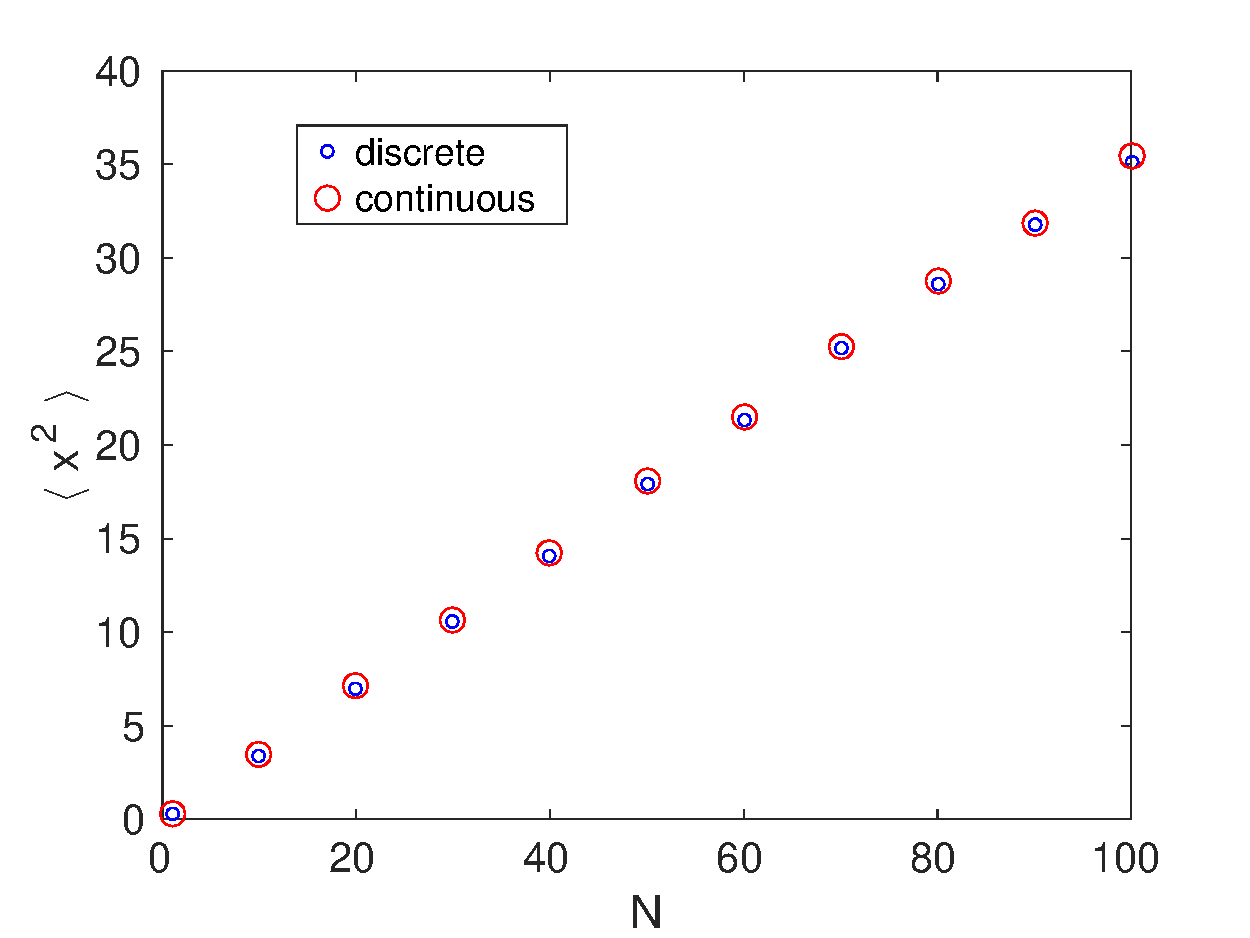
\includegraphics[width=0.5\textwidth]{diffuseDiscreteContinuous}
\caption{Numerical experiment of MSD.  We plot the $\langle
x^2\rangle$ as a function of the number of disk collisions, i.e.
topological length. Blue dots are obtained from the discrete
map, and red circles are results from the full flow. Each point
is calculated using 35000 trajectories.}
\label{fig-disvscont}
\end{figure}
